\begin{homeworkProblem}
    (1.2, Taylor) Two vectors are given as $\textbf{b} = (1,2,3)$ and $\textbf{c} = (3,2,1)$. Find $\textbf{b}+\textbf{c}$, $5\textbf{b}-2\textbf{c}$, $\textbf{b}\cdot \textbf{c}$, and $\textbf{b}\times \textbf{c}$.

    \begin{callout}{Solution:}

        \begin{enumerate}[i.]
            \item $(1,2,3)+(3,2,1) = (4,4,4)$
            \item $(5,10,15)-(6,4,2) = (-1,6,13)$
            \item $(1,2,3)\cdot(3,2,1) = 3+4+3 = 10$ 
            \item 
                \begin{align*}
                    \left| \begin{array}{ccc} 
                        \hat{\textbf{i}} & \hat{\textbf{j}} & \hat{\textbf{k}} \\ 
                        1 & 2 & 3 \\ 
                        3 & 2 & 1
                    \end{array} \right|
                    &= (2-6)\hat{\textbf{i}} - (1-9)\hat{\textbf{j}} + (2-6)\hat{\textbf{k}} \\ 
                    &= (-4, 8, -4)
                \end{align*}
        \end{enumerate}

    \end{callout}

\end{homeworkProblem}

\newpage
\begin{homeworkProblem}
    (1.5, Taylor) Find the angle between a body diagonal of a cube and any one of its face diagonals. [Hint: choose a cube with side 1 and with one corner at 0 and the opposite corner at the point (1,1,1). Write down the vector that represents a body diagonal and another that represents a face diagonal, then find the angle between them as in problem 1.4.]

    \begin{callout}{Solution:}

        I will work with diagonal vector $\alpha = (1,1,1)$ and vertex at $\beta = (1,1,0)$. The angle between them is given by the following definition of the dot product
        $$|\alpha||\beta|\cos\theta = \alpha \cdot \beta$$
        \begin{align*}
            |\alpha| &= \sqrt{ 3 } \\ 
            |\beta| &= \sqrt{ 2 } \\ 
            \alpha \cdot \beta &= 2
        \end{align*}
        This gives
        $$\theta = \cos\left( \frac{2}{\sqrt{6}} \right)$$

    \end{callout}

\end{homeworkProblem}

\newpage
\begin{homeworkProblem}
    (1.6, Taylor) By evaluating their dot product, find the values of the scalar $s$ for which the two vectors $\textbf{b}=\hat{\textbf{x}}+s \hat{\textbf{y}}$ and $\textbf{c}=\hat{\textbf{x}}-s \hat{\textbf{y}}$ are orthagonal. (remember that two vectors are orthagonal if and only if their dot product is zero.) Explain your answers with a sketch.

    \begin{callout}{Solution:}

        \begin{align*}
            (1,s) \cdot (1,-s) &= 0 \\ 
            1 - s^2 &= 0 \\ 
            s^2 &= 1
        \end{align*}

        This implies $s$ equals $\pm 1$.

        \begin{center}
            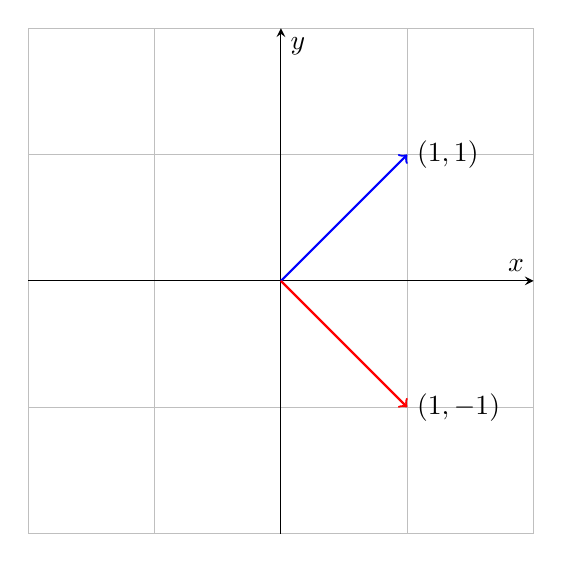
\begin{tikzpicture}
                \begin{axis}[
                        axis lines = middle,
                        grid = both,
                        xlabel = \(x\),
                        ylabel = \(y\),
                        xmin = -2, xmax = 2,
                        ymin = -2, ymax = 2,
                        width = 8cm,
                        height = 8cm,
                        ticks = none
                    ]
                    % Plot the vectors
                    \addplot[blue, thick,->] coordinates {(0,0) (1,1)};
                    \addplot[red, thick,->] coordinates {(0,0) (1,-1)};

                    % Add labels
                    \node at (axis cs:1,1) [anchor=west] {\( (1,1) \)};
                    \node at (axis cs:1,-1) [anchor=west] {\( (1,-1) \)};
                \end{axis}
            \end{tikzpicture}
        \end{center}

    \end{callout}

\end{homeworkProblem}

\newpage
\begin{homeworkProblem}
    (1.19, Taylor) If \textbf{r}, \textbf{v}, \textbf{a} denote the position, velocity, and acceleration of a particle, prove that
    $$\frac{d}{dt}[\textbf{a}\cdot(\textbf{v} \times \textbf{r})] = \dot{\textbf{a}}\cdot (\textbf{v}\times \textbf{r})$$

    \begin{callout}{Solution:}

        \begin{align*}
            \frac{d}{dt}[\textbf{a}\cdot(\textbf{v} \times \textbf{r})] = \left[ \frac{d}{dt}(\mathbf{a}) \cdot (\mathbf{v} \times \mathbf{r}) \right] + \left[ (\mathbf{a})\cdot\frac{d}{dt}(\mathbf{v}\times \mathbf{r}) \right] \tag{1}
        \end{align*}

        The product rule applied to cross products makes the right hand side of the sum:

        \begin{align*}
            &= (\textbf{a}) \cdot \left( \frac{d \textbf{r}}{dt}\times \textbf{v} + \textbf{r} \times \frac{d \textbf{v}}{dt} \right) \\
            &= (\textbf{a}) \cdot \left( \cancelto{0}{\textbf{v} \times \textbf{v}} + \textbf{r} \times \textbf{a} \right)
        \end{align*}

        Because $\textbf{r}\times \textbf{a}$ results in a vector orthagonal to $\textbf{a}$, the resulting dot product here will be zero. As a result the only part of equation (1) which remains is the left side of the sum. Therefore:

        $$\frac{d}{dt}[\textbf{a}\cdot(\textbf{v} \times \textbf{r})] = \dot{\textbf{a}}\cdot (\textbf{v}\times \textbf{r})$$
    \end{callout}

\end{homeworkProblem}

\newpage
\begin{homeworkProblem}
    (1.22, Taylor) The two vectors \textbf{a} and \textbf{b} lie in the $xy$ plane and make angles $\alpha$ and $\beta$ with the $x$ axis. \textbf{(a)} By evaluating $\textbf{a}\cdot \textbf{b}$ in two ways [namely using (1.6) and (1.7)] prove the well-known trig identity
    $$\cos(\alpha -\beta)=\cos \alpha \cos \beta + \sin \alpha \sin \beta.$$
    \textbf{(b)} By similarly evaluating $\textbf{a} \times \textbf{b}$ prove that
    $$\sin(\alpha - \beta) = \sin \alpha \cos \beta - \cos \alpha \sin \beta.$$

    \begin{callout}{Solution:}

        \begin{enumerate}[(a)]
            \item The relevant trig identities here are:
                \begin{align*}
                    \textbf{a} \cdot \textbf{b} &= |a||b| \cos(\alpha - \beta) \tag{1} \\ 
                    \textbf{a} \cdot \textbf{b} &= a_x b_x + a_y b_y \tag{2} \\ 
                    &= (|a|\cos(\alpha)) (|b|\cos(\beta)) + (|a|\sin(\alpha)) (|b|\sin(\beta)) \\ 
                    &= |a||b|(\cos(\alpha)\cos(\beta)+\sin(\alpha)\sin(\beta))
                \end{align*}

                Equating (1) and (2) allows us to get a relation in terms of angles alone:

                $$\cancel{|a||b|}\cos(\alpha -\beta) = \cancel{|a||b|}(\cos \alpha \cos \beta + \sin \alpha \sin \beta)$$

            \item Recall that components given in terms of $(r,\theta)$ in cartesian coordinates are $(|x|\cos \theta , |y|\sin\theta)$. The cross product between two such vectors is therefore:

                \begin{align*}
                    \textbf{a} \times \textbf{b} =
                    \left| \begin{array}{ccc} \hat{\textbf{i}} & \hat{\textbf{j}} & \hat{\textbf{k}} \\ |a|\cos \alpha  & |a| \sin \alpha & 0 \\ |b|\cos \beta & |b| \sin \beta & 0 \end{array} \right| 
                        = \{(|a||b|\cos \alpha \sin \beta) - |a||b|(\sin \alpha \cos \beta )\}\hat{\textbf{z}} \tag{3}
                \end{align*}

                To complete the proof we need to utilize another definition of the cross product which I have never seen until now:

                \begin{align*}
                    \textbf{a} \times \textbf{b} = |a||b|\sin(\alpha -\beta)(-\hat{\textbf{z}}) \tag{4}
                \end{align*}

                Equating (3) and (4) leaves us with:

                $$\sin(\alpha - \beta) = \sin \alpha \cos \beta - \cos \alpha \sin \beta$$

        \end{enumerate}
           \end{callout}
\end{homeworkProblem}
